
\documentclass[xcolor={usenames,dvipsnames},12pt,presentation,aspectratio=169]{beamer}

\usepackage[utf8]{inputenc}
\usepackage{fontawesome}
\usepackage[brazilian]{babel}
\usepackage{verbatim}
\usepackage{graphicx}
\usepackage{xspace}
\usepackage{amsthm}
\usepackage{url}
\usepackage{array}
\usepackage{hyperref}
\usepackage{times,mathptmx}
\usepackage{pdfpages}
\usepackage{mdframed}
\usepackage{tikz}
\usepackage{alltt}
\usepackage{minted}
%\usepackage{times}
%\usepackage[usenames,dvipsnames]{xcolor}
%\usepackage[usenames,dvipsnames]{color}
%\usepackage{color}

\usetikzlibrary{arrows,shapes}

\usetheme{Madrid}
%\usetheme{Boadilla}
%\usetheme{Darmstadt}
%\usetheme{Frankfurt}
%\usetheme{CambridgeUS}
%\usetheme{AnnArbor}
%\usecolortheme{beaver}
%\usecolortheme{seahorse}
%\usecolortheme{seagull}
\usecolortheme[named=BrickRed]{structure}

\setbeamercovered{transparent}

\setbeamertemplate{footline}[frame number]
%\setbeamertemplate{navigation symbols}{}
%\setbeamersize{text margin left=1em,text margin right=1em}

\newcommand{\titulo}{Programação Paralela com MPI}
\newcommand{\disciplina}{ELC139 - Programação Paralela}
\newcommand{\nome}{João Vicente Ferreira Lima (UFSM)}

\lecture[1]{\aula}{aula01}
\def\lecturename{\aula}

\newcommand{\Red}[1]{{\color{red}#1}}
\newcommand{\red}[1]{{\color{red}#1}}
\newcommand{\Blue}[1]{{\color{blue}#1}}
\newcommand{\blue}[1]{{\color{blue}#1}}

\newcommand{\PBS}[1]{\let\temp=\\#1\let\\=\temp}
\newcommand{\RRCOL}{\PBS\raggedright\hspace{0pt}}

\newcommand{\p}[1]{\texttt{#1}}
\newenvironment{code}{%
  \begin{alltt}%
  }{%
  \end{alltt}%
}

\makeatletter
%\setbeamertemplate{headline}{}
% {%
%   \leavevmode%
%   \@tempdimb=2.4375ex%
%   \ifnum\beamer@subsectionmax<\beamer@sectionmax%
%     \multiply\@tempdimb by 4%
%   \else%
%     \multiply\@tempdimb by\beamer@subsectionmax%
%   \fi%
%   \ifdim\@tempdimb>0pt%
%     \advance\@tempdimb by 1.125ex%
%     \begin{beamercolorbox}[wd=.5\paperwidth,ht=\@tempdimb]{section in head/foot}%
%       \vbox to\@tempdimb{\vfil\insertsectionnavigation{.5\paperwidth}\vfil}%
%     \end{beamercolorbox}%
%     \begin{beamercolorbox}[wd=.45\paperwidth,ht=\@tempdimb]{subsection in head/foot}%
%       \vbox
%       to\@tempdimb{\vfil\insertsubsectionnavigation{.45\paperwidth}\vfil}%
%     \end{beamercolorbox}%
%     \begin{beamercolorbox}[wd=.05\paperwidth,ht=\@tempdimb]{subsection in head/foot}%
%       \vbox
%       to\@tempdimb{\vfil\hfil\insertframenumber\vfil\vfil}%
%     \end{beamercolorbox}%
%   \fi%
% }

\def\dohead{\beamer@headcounter=4\relax\beamer@headcounter=1\loop\ifnum\beamer@headcounter<\beamer@totalheads%
  \advance\beamer@headcounter by1\relax%
  \csname @@head\the\beamer@headcounter\endcsname\repeat}

\makeatother

\title[\titulo]{\titulo}

\subtitle{\disciplina}

\author[João V. F. Lima]{\nome}

%\institute[UFSM]{Departamento de Linguagens e Sistemas de Computação \\ Universidade Federal de Santa Maria \\ \url{jvlima@inf.ufsm.br} \\ \url{http://www.inf.ufsm.br/~jvlima}}
\institute[UFSM]{Universidade Federal de Santa Maria \\ \url{jvlima@inf.ufsm.br} \\ \url{http://www.inf.ufsm.br/~jvlima}}
\date{2023/1}

\graphicspath{{.}{figs/}}

\logo{ 
\includegraphics[height=1.5cm,width=1.5cm,keepaspectratio]{logo_inf}    
        
\includegraphics[height=1.5cm,width=1.5cm,keepaspectratio]{logo_ufsm} }

%\titlegraphic{
%	
\includegraphics[width=2cm]{logo_ufsm}
%  \hspace{1cm}
%	
\includegraphics[width=2cm]{logo_inf}
%}

\newtheorem{mydef}{Definição}[section]
%\newtheorem{myteo}{Teorema}[section]
%------------------------------------------------------------------------------
%\newcommand{\xkaapi}{XKaapi\xspace}
%------------------------------------------------------------------------------
% Typesetting Listings
\usepackage{listings}
\lstset{
  language=C,
  %basicstyle=\scriptsize\ttfamily,
  %basicstyle=\normalsize\ttfamily,
  basicstyle=\small\ttfamily,
  %basicstyle=\footnotesize\ttfamily,
  %aboveskip=0pt,
  %belowskip=0pt,
  %mathescape=false,
  columns=fullflexible,
  %numbers=none,
  numbers=left,
  numbersep=5pt,
%  showtabs=true,
%  showspaces=true,
  frame=tb,
  breaklines=true
}
%------------------------------------------------------------------------------
%\lstset{commentstyle=\color{blue}}
%\lstset{stringstyle=\ttfamily}
%\lstset{ classoffset=1, 
%            morekeywords={kaapi,omp,task,data,alloca, declare, reduction, identity, parallel,sync,taskwait,cilk,spawn,tbb,css,cilk\_spawn,cilk\_sync,cilk\_for,offload},
%            keywordstyle=\color{Red}\bfseries
%           }
%\lstset{ classoffset=2, 
%            morekeywords={value,read,write,readwrite,reduction,untied,firstprivate,TaskBodyCPU,TaskBodyGPU,ka,Signature,RW,CW,range2d\_r,range2d\_rw,range2d,Spawn,Fork,Shared\_w,Shared\_r,Shared,a1,target,device,copyin,copyout,input,implements,copy\_deps,RPWP,range2d\_rpwp,rangeindex,Memory,Register,SetStaticSched,Sync,Unregister,Community,System,join\_community,SpawnMain,leave,initialize,terminate,logfile,array,SetArch,ArchHost,ArchCUDA,W,R,gpuStream,pointer\_w,pointer\_r,pointer\_cw,pointer},
%            keywordstyle=\color{Blue}\bfseries
%           }
%\lstset{ classoffset=3, 
%            morekeywords={storage,ld},
%            keywordstyle=\bfseries
%           }
%\lstset{ classoffset=4, 
%            morekeywords={in,out,inout,cout,concurrent},
%            keywordstyle=\color{Red}\bfseries
%           }
%           
%\lstset{classoffset=0, showstringspaces=false}
%------------------------------------------------------------------------------
\mdfsetup{
  backgroundcolor=gray!10,
%  roundcorner=10pt,
}
%------------------------------------------------------------------------------
\newcommand{\restorefootline}{\setbeamertemplate{navigation symbols}{}}
%\newcommand{\setfootline}[1]{\setbeamertemplate{navigation symbols}{\textcolor{black}{\textbf{#1}}}}
\newcommand{\includeslides}[4]{%
%  \setfootline{#1}%
  {
    \setbeamercolor{background canvas}{bg=}
    \includepdf[pages={#1},%
    pagecommand={},
%    pagecommand={\begin{frame}[default]{}\end{frame}},
%    #4,%
    turn=false,noautoscale=false,column=false,columnstrict=false,openright=false,frame=false]{#2}%
  }
  %\restorefootline%
}
%------------------------------------------------------------------------------
\begin{document}

\begin{frame}
%  \titlepage
  \maketitle
%  \mode<presentation>
%  {
%    \begin{columns}
%      \begin{column}{0.5\textwidth}
%      \raggedleft
%	
\includegraphics[width=2cm]{logo_ufsm}
%      \end{column}
%      \begin{column}{0.5\textwidth}
%	
\includegraphics[width=2cm]{logo_inf}
%      \end{column}
%    \end{columns}
%  }
\end{frame}

\begin{frame}
    \frametitle{Outline}
    \tableofcontents[hideallsubsections]
%    \tableofcontents
\end{frame}

\AtBeginSection{
  \begin{frame}
    \frametitle{Outline}
    \tableofcontents[currentsection,hideothersubsections]
  \end{frame}
}


%%%%%%%%%%%%%%%%%%%%%%%%%%%%%%%%%%%%%%%%%%%%%%%%%%%%%%%%%%%%%%%%%%%%%%%%%%%%%%
\section{Primeiros Passos}
%%%%%%%%%%%%%%%%%%%%%%%%%%%%%%%%%%%%%%%%%%%%%%%%%%%%%%%%%%%%%%%%%%%%%%%%%%%%%%%
%------------------------------------------------------------------------------
\begin{frame}
  \frametitle{Sistema de memória distribuída}
  \vspace{-4mm}
  \begin{center}
	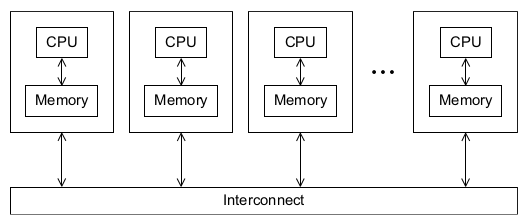
\includegraphics[width=0.8\textwidth]{distribuido.png}
  \end{center}
  \vfill
  {\tiny Introduction to Parallel Computing, Grama et al, 2003.}
\end{frame}
%------------------------------------------------------------------------------
\begin{frame}
  \frametitle{Sistema de memória compartilhada}
  \vspace{-4mm}
  \begin{center}
	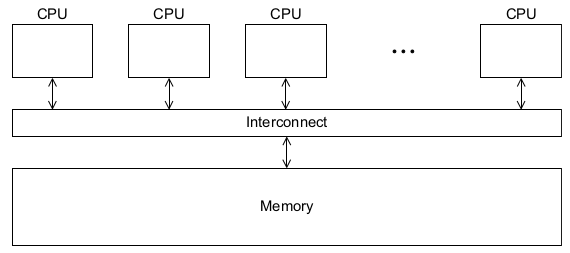
\includegraphics[width=0.8\textwidth]{compartilhado.png}
  \end{center}
  \vfill
  {\tiny Introduction to Parallel Computing, Grama et al, 2003.}
\end{frame}
%%%%%%%%%%%%%%%%%%%%%%%%%%%%%%%%%%%%%%%%%%%%%%%%%%%%%%%%%%%%%%%%%%%%%%%%%%%%%%
\section{Olá mundo}
%%%%%%%%%%%%%%%%%%%%%%%%%%%%%%%%%%%%%%%%%%%%%%%%%%%%%%%%%%%%%%%%%%%%%%%%%%%%%%%
%------------------------------------------------------------------------------
\begin{frame}[fragile]
  \frametitle{Olá mundo}
  
  \begin{center}
\begin{minipage}{0.9\textwidth}
  \begin{minted}[linenos, frame=lines]{C}
#include <stdio.h>

int main(void)
{
  printf("hello, world\n");

  return 0;
}
  \end{minted}
\end{minipage}
\end{center}
\end{frame}
%---------------------------------------------------------------
\begin{frame}[fragile]
  \frametitle{Olá mundo}
  
\begin{center}
\begin{minipage}{0.9\textwidth}
  \begin{minted}[linenos, frame=lines]{C}
#include <stdio.h>
#include <mpi.h>

int main(void)
{
  /* Nenhuma chamada MPI pode acontecer antes */
  MPI_Init(NULL, NULL);

  /* Chamadas MPI */

  MPI_Finalize();
  /* Nenhuma chamada MPI pode acontecer depois */
  return 0;
}
  \end{minted}
\end{minipage}
\end{center}
\end{frame}
%------------------------------------------------------------------------------
\begin{frame}[fragile]
  \frametitle{Compilação}
  \begin{center}  
  \begin{minipage}{0.9\textwidth}
    \begin{minted}[linenos, frame=lines]{Bash}
$ mpicc -g -Wall -o mpi_hello mpi_hello.c
    \end{minted}
  \end{minipage}
  \end{center}
%
\begin{itemize}
  \item \texttt{mpicc} é um \emph{wrapper} (script)
  \begin{itemize}
    \item \texttt{mpicc --showme} -- Mostra o comando real executado.
  \end{itemize}
  \item As outras opções e flags são passadas diretamento ao compilador
\end{itemize}
\end{frame}
%------------------------------------------------------------------------------
\begin{frame}[fragile]
  \frametitle{Execução}
  \begin{center}  
  \begin{minipage}{0.9\textwidth}
    \begin{minted}[linenos, frame=lines]{Bash}
$ mpiexec -n <n. de processos> <executável>
    \end{minted}
  \begin{minted}[linenos, frame=lines]{Bash}
$ mpiexec -n 1 ./mpi_hello

$ mpiexec -n 4 ./mpi_hello
  \end{minted}
  \end{minipage}
  \end{center}
%
\begin{itemize}
  \item \texttt{mpiexec} também é um \emph{wrapper} (script) para executar o programa
  \item Uma vasta lista de opções disponíveis
  \begin{itemize}
    \item Processadores e cores, threads por processo, variáveis de ambientes, etc.
  \end{itemize}
\end{itemize}
\end{frame}
%------------------------------------------------------------------------------
%------------------------------------------------------------------------------
\begin{frame}[fragile]
  \frametitle{MPI}
\begin{block}{\mintinline{C}{MPI_Init}}
  \begin{itemize}
    \item Inicia o MPI, fazendo o setup inicial.
  \end{itemize}
  \begin{center}  
    \begin{minipage}{0.9\textwidth}
      \begin{minted}[linenos, frame=lines]{C}
int MPI_Init(
        int* argc,    /* in/out */
        char*** argv  /* in/out */
);
      \end{minted}
    \end{minipage}
    \end{center}
    \begin{itemize}
      \item \texttt{argc} e \texttt{argv} são ponteiros recebidos pela \texttt{main}.
    \end{itemize}  
  \end{block}
%
\begin{block}{\mintinline{C}{MPI_Finalize}}
  \begin{itemize}
    \item Sinalize que o programa terminou e libera recursos
  \end{itemize}
  \begin{center}  
    \begin{minipage}{0.9\textwidth}
      \begin{minted}[linenos, frame=lines]{C}
int MPI_Finalize(void);
      \end{minted}
    \end{minipage}
    \end{center}
  \end{block}
\end{frame}
%------------------------------------------------------------------------------
\begin{frame}[fragile]
  \frametitle{Olá mundo}
\begin{center}
\begin{minipage}{0.95\textwidth}
  \begin{minted}[linenos, fontsize=\small, breaklines=true, frame=lines]{C}
#include <stdio.h>
#include <mpi.h>

int main(void)
{
  int rank, comm_size;
  MPI_Init(NULL, NULL);

  MPI_Comm_size(MPI_COMM_WORLD, &comm_size);
  MPI_Comm_rank(MPI_COMM_WORLD, &rank);

  printf ("Hello from process %d of %d!\n", rank, comm_size);

  MPI_Finalize();
  return 0;
}
  \end{minted}
\end{minipage}
\end{center}
\end{frame}
%------------------------------------------------------------------------------
\begin{frame}[fragile]
  \frametitle{Executando}
\begin{center}
\begin{minipage}{0.95\textwidth}
  \begin{minted}[linenos, fontsize=\small, breaklines=true,   frame=lines]{text}
$ mpiexec -n 1 ./hello_mpi
Hello from process 0 of 1!
$ mpiexec -n 2 ./hello_mpi
Hello from process 0 of 2!
Hello from process 1 of 2!
$ mpiexec -n 6 ./hello_mpi
There are not enough slots available in the system to satisfy 
the 6 slots that were requested by the application:

  ./hello_mpi

Either request fewer slots for your application, or make more 
slots available for use.
  \end{minted}
\end{minipage}
\end{center}
\end{frame}
%------------------------------------------------------------------------------
\begin{frame}[fragile]
  \frametitle{Comunicadores}
%
\begin{itemize}
  \item Um comunicador (\emph{communicator}) é um conjunto de processos que podem mandar mensagens entre si
  \item A função \mintinline{C}{MPI_Init} é definir um comunicador que consiste em todos os processos criados quando o programa é executado
  \item O comunicador é o \mintinline{C}{MPI_COMM_WORLD} do tipo \mintinline{C}{MPI_Comm}
  \item Outro comunidor especial é o \mintinline{C}{MPI_COMM_SELF}
\end{itemize}
\end{frame}
%------------------------------------------------------------------------------
\begin{frame}[fragile]
  \frametitle{Comunicadores}
  \vspace{-2mm}
\begin{block}{\mintinline{C}{MPI_Comm_size}}
  \begin{itemize}
    \item Consulta o número de processos no comunidador
  \end{itemize}
  \begin{center}  
    \begin{minipage}{0.9\textwidth}
      \begin{minted}[linenos, frame=lines]{C}
int MPI_Comm_size(
        MPI_Comm comm,  /* in */
        int* size       /* out */
);
      \end{minted}
    \end{minipage}
    \end{center}
  \end{block}
%
\begin{block}{\mintinline{C}{MPI_Comm_rank}}
  \begin{itemize}
    \item Retorna o rank do processo que chamou a função
  \end{itemize}
  \begin{center}  
    \begin{minipage}{0.9\textwidth}
      \begin{minted}[linenos, frame=lines]{C}
int MPI_Comm_rank(
          MPI_Comm comm,  /* in */
          int* rank       /* out */
  );  
      \end{minted}
    \end{minipage}
    \end{center}
  \end{block}
\end{frame}
%------------------------------------------------------------------------------
%\begin{frame}[fragile]
%  \frametitle{Olá mundo}
%\begin{center}
%\begin{minipage}{0.95\textwidth}
%  \begin{minted}[linenos, fontsize=\small, breaklines=true, frame=lines]{C}
%int main (int argc, char *argv[])
%{
%  int   rank, comm_size;
%  char hostname[MPI_MAX_PROCESSOR_NAME];
%  char msg[MPI_MAX_PROCESSOR_NAME+30];
%    
%  MPI_Init(NULL, NULL);
%  MPI_Comm_size(MPI_COMM_WORLD, &comm_size);
%  MPI_Comm_rank(MPI_COMM_WORLD, &rank);
%  MPI_Get_processor_name(hostname, &len);
%  if(rank != 0){
%    sprintf(msg, "Hello from %s rank %d", hostname, rank);
%    MPI_Send(msg, strlen(msg)+1, MPI_CHAR, 0, 0, MPI_COMM_WORLD);
%  } else {
%    for(int p = 1; p < comm_size; p++){
%      MPI_Recv(msg, MPI_MAX_PROCESSOR_NAME+30, MPI_CHAR, p, 0, MPI_COMM_WORLD, MPI_STATUS_IGNORE);
%      printf("%s\n", msg);
%    }
%  }
%  MPI_Finalize();
%  return 0;
%}    
%  \end{minted}
%\end{minipage}
%\end{center}
%\end{frame}
%------------------------------------------------------------------------------
\begin{frame}[fragile]
  \frametitle{Olá mundo}
\begin{center}
\begin{minipage}{0.95\textwidth}
  \begin{minted}[linenos, fontsize=\small, breaklines=true, frame=lines]{C}
int main (int argc, char *argv[])
{
  int   rank, comm_size, len;
  char hostname[MPI_MAX_PROCESSOR_NAME];
  char msg[MPI_MAX_PROCESSOR_NAME+30];
    
  MPI_Init(NULL, NULL);
  MPI_Comm_size(MPI_COMM_WORLD, &comm_size);
  MPI_Comm_rank(MPI_COMM_WORLD, &rank);
  MPI_Get_processor_name(hostname, &len);
  ...
  \end{minted}
\end{minipage}
\end{center}
\end{frame}
%------------------------------------------------------------------------------
\begin{frame}[fragile]
  \frametitle{Olá mundo}
\begin{center}
\begin{minipage}{0.95\textwidth}
  \begin{minted}[linenos, fontsize=\small, breaklines=true, frame=lines]{C}
  ...
  if(rank != 0){
    sprintf(msg, "Hello from %s rank %d", hostname, rank);
    MPI_Send(msg, strlen(msg)+1, MPI_CHAR, 0, 0, MPI_COMM_WORLD);
  } else {
    for(int p = 1; p < comm_size; p++){
      MPI_Recv(msg, MPI_MAX_PROCESSOR_NAME+30, MPI_CHAR, p, 0, MPI_COMM_WORLD, MPI_STATUS_IGNORE);
      printf("%s\n", msg);
    }
  }
  MPI_Finalize();
  return 0;
}    
  \end{minted}
\end{minipage}
\end{center}
\end{frame}
%------------------------------------------------------------------------------
\begin{frame}[fragile]
  \frametitle{Comunicadores}
  \vspace{-2mm}
\begin{block}{\mintinline{C}{MPI_Send}}
  \begin{center}  
    \begin{minipage}{0.9\textwidth}
      \begin{minted}[linenos, frame=lines]{C}
int MPI_Send(
    const void   *buf,     /* in */
    int          count,    /* in */
    MPI_Datatype datatype, /* in */
    int          dest,     /* in */
    int          tag,      /* in */
    MPI_Comm     comm      /* in */
);
      \end{minted}
    \end{minipage}
    \end{center}
  \end{block}
\end{frame}
%------------------------------------------------------------------------------
\begin{frame}
  \frametitle{Comunicadores}
  \vspace{-4mm}
  \begin{center}
	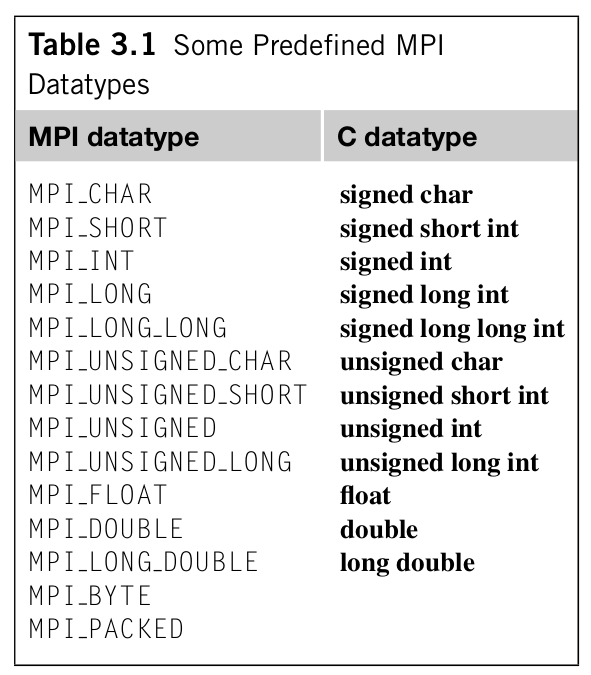
\includegraphics[width=0.4\textwidth]{datatype.png}
  \end{center}
  \vfill
  {\tiny Introduction to Parallel Computing, Grama et al, 2003.}
\end{frame}
%------------------------------------------------------------------------------
\begin{frame}[fragile]
  \frametitle{Comunicadores}
  \vspace{-2mm}
\begin{block}{\mintinline{C}{MPI_Recv}}
  \begin{center}  
    \begin{minipage}{0.9\textwidth}
      \begin{minted}[linenos, frame=lines]{C}
int MPI_Recv(
    void         *buf,     /* out */
    int          count,    /* in */
    MPI_Datatype datatype, /* in */
    int          source,   /* in */
    int          tag,      /* in */
    MPI_Comm     comm,     /* in */
    MPI_Status   *status  /* out */
);
      \end{minted}
    \end{minipage}
    \end{center}
  \end{block}
\end{frame}
%------------------------------------------------------------------------------
\begin{frame}[fragile]
  \frametitle{Comunicação}
\begin{itemize}
  \item Vários parâmetros precisam casar (\emph{match}) para uma mensagem ser entregue
  \item Assumindo que \texttt{p1} envia uma mensagem para \texttt{p2}
  \begin{itemize}
    \item \mintinline{C}{comm1 == comm2} 
    \item \mintinline{C}{tag1 == tag2} 
    \item \mintinline{C}{dest == p2} 
    \item \mintinline{C}{source == p1} 
  \end{itemize} 
\end{itemize}
%
\begin{center}
\begin{minipage}{0.95\textwidth}
  \begin{minted}[linenos, fontsize=\small, breaklines=true, frame=lines]{C}
int MPI_Send(const void *send_buf, int send_size, MPI_Datatype send_type, int dest, int tag1, MPI_Comm comm1);

int MPI_Recv(void *rec_buf, int rec_size, MPI_Datatype rec_type, int source, int tag2, MPI_Comm comm2, MPI_Status *status);
  \end{minted}
\end{minipage}
\end{center}
\end{frame}
%------------------------------------------------------------------------------
\begin{frame}[fragile]
  \frametitle{Comunicação}
\begin{itemize}
  \item As condições anteriores não garantem o sucesso do envio da mensagem.
  \item Os pares adicionais são:
  \begin{itemize}
    \item \mintinline{C}{send_type == rec_type}
    \item \mintinline{C}{rec_size >= send_size }
  \end{itemize}
  
\end{itemize}
%
\begin{center}
\begin{minipage}{0.95\textwidth}
  \begin{minted}[linenos, fontsize=\small, breaklines=true, frame=lines]{C}
int MPI_Send(const void *send_buf, int send_size, MPI_Datatype send_type, int dest, int tag1, MPI_Comm comm1);

int MPI_Recv(void *rec_buf, int rec_size, MPI_Datatype rec_type, int source, int tag2, MPI_Comm comm2, MPI_Status *status);
      \end{minted}
\end{minipage}
\end{center}
\end{frame}
%------------------------------------------------------------------------------
\begin{frame}[fragile]
  \frametitle{Comunicação}
\begin{itemize}
  \item O \mintinline{C}{MPI_Recv} recebe também a variável do tipo \mintinline{C}{MPI_Status} contendo
  \begin{itemize}
    \item O tamanho da mensagem 
    \item A origem da mensagem \mintinline{C}{MPI_SOURCE}
    \item A tag da mensagem \mintinline{C}{MPI_TAG}
    \item Erro se acontecer \mintinline{C}{MPI_ERROR}
  \end{itemize}
  \item Os parâmetros \mintinline{C}{MPI_ANY_SOURCE} e \mintinline{C}{MPI_ANY_TAG} permitem aceitar mensagens de qualquer fonte com qualquer tag
\end{itemize}
%
\end{frame}
%------------------------------------------------------------------------------
\begin{frame}[fragile]
  \frametitle{Comunicação}
\begin{center}
  \begin{minipage}{0.95\textwidth}
    \begin{minted}[linenos, fontsize=\small, breaklines=true, frame=lines]{C}
MPI_Status status;
MPI_Recv(rec_buf, rec_size, rec_type, MPI_ANY_SOURCE, MPI_ANY_TAG, rec_comm, &status);

int src = status.MPI_SOURCE;
int tag = status.MPI_TAG;
int count;
MPI_Get_count(&status, rec_type, &count);
        \end{minted}
  \end{minipage}
  \end{center}
  
\end{frame}
%------------------------------------------------------------------------------
\begin{frame}[plain]{}
  \begin{center}
    \vspace{2cm}
    \Large{https://joao-ufsm.github.io/par2023a/}
    
    \vspace{1cm}
    
\includegraphics[width=2cm]{logo_ufsm}
    \hspace{0.5cm}
    
\includegraphics[width=2cm]{logo_inf}
  \end{center}
\end{frame}
%------------------------------------------------------------------------------

\end{document}
